% figure.tex
\documentclass[tikz,border=2pt]{standalone}
\usepackage{amsmath}
\usepackage{tikz}
\usetikzlibrary{plotmarks,patterns,intersections,calc}

\begin{document}
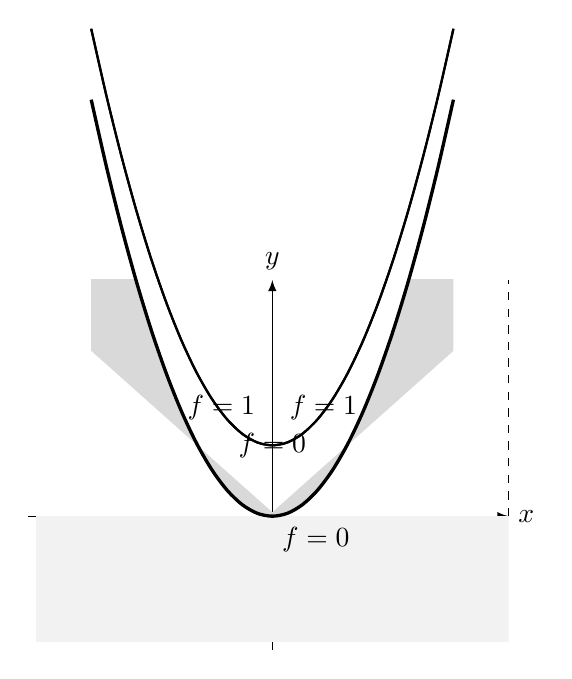
\begin{tikzpicture}[scale=1.0, >=latex]

  % 画布参数
  \def\xmin{-3.0}
  \def\xmax{3.0}
  \def\ymin{-1.6}
  \def\ymax{3.0}

  % 坐标轴
  \draw[->] (0,\ymin-0.1) -- (0,\ymax) node[above] {$y$};
  \draw[->] (\xmin-0.1,0) -- (\xmax,0) node[right] {$x$};
  \node[below left] at (0,0) {O};

  % 定义抛物线路径(从 -2 到 2)
  \draw[domain=-2.0:2.0,smooth,variable=\x,thick] 
    plot ({\x},{\x*\x}) coordinate[pos=0.5](midparabola);

  % 两条倾斜边界(用直线近似图中“外侧曲线”的倾向)
  \path[name path=leftline]  (-2.3,2.1) -- (0,0.05);
  \path[name path=rightline] (2.3,2.1)  -- (0,0.05);

  % 抛物线路径用于计算交点(扩展一点以保证交点存在)
  \path[name path=parab] plot[domain=-2.3:2.3,smooth,variable=\x] ({\x},{\x*\x});

  % 计算交点(leftline 与 parabola 的上交点)
  \path[name intersections={of=leftline and parab, name=I}];
  \path[name intersections={of=rightline and parab, name=J}];

  % 如果 intersections 没找到恰好点也会取到最接近的点 —— 用作闭合边界
  % 构造上边界(由左直线到右直线)和下边界(抛物线,从右到左)形成闭合区域
  \begin{scope}
    \clip (\xmin,\ymin) rectangle (\xmax,\ymax); % 限制绘制范围
    % 填充上部阴影:区域由左线 -> 交点上 -> 抛物线沿到另一个交点 -> 右线 回到起点
    \fill[gray!30] 
      % 从左直线高处开始(保证闭合)
      (-2.3,2.1) -- (0,0.05) -- (2.3,2.1) 
      -- plot[domain=2.3:-2.3,smooth,variable=\x] ({\x},{\x*\x}) -- cycle;
  \end{scope}

  % 下方(x 轴以下)浅色矩形作为“f=0区域”,并裁切到画布
  \begin{scope}
    \clip (\xmin,\ymin) rectangle (\xmax,0);
    \fill[gray!10] (\xmin,\ymin) rectangle (\xmax,0);
  \end{scope}

  % 重画抛物线以覆盖阴影边界(更清晰)
  \draw[domain=-2.3:2.3,smooth,variable=\x, very thick] plot ({\x},{\x*\x});

  % 在左右侧画两条近似“f=1”的曲线(用稍向外的抛物线作为示意)
  \draw[domain=-2.3:2.3,smooth,variable=\x, thick] plot ({\x},{\x*\x + 0.9});
  \draw[domain=-2.3:2.3,smooth,variable=\x, thick] plot ({\x},{\x*\x + 0.9});

  % 下方与上方文字标注
  \node at (0,0.9) {$f=0$};         % 在抛物线附近标注 f=0
  \node[anchor=south west] at (-1.2,1.1) {$f=1$}; % 左侧 f=1 标注
  \node[anchor=south east] at (1.2,1.1) {$f=1$};  % 右侧 f=1 标注

  % 辅助细节:在抛物线顶点附近再标一个 f=0(靠近原图)
  \node[below right] at (0,-0.02) {$f=0$};

  % 可选:画虚线表示某些垂直参考线(如图中竖线)
  \draw[dashed] (3.0,0) -- (3.0,3.0); % 仅作示意(可删)

\end{tikzpicture}
\end{document}

